\documentclass[12pt]{report}
\usepackage[margin=1cm, top=1.5cm, bottom=1.5cm]{geometry}
\usepackage{minted}
\usepackage{xcolor}
\usepackage{tcolorbox}
\usepackage{babel}
\usepackage[T1]{fontenc}
\usepackage{textcomp}
\usepackage{titlesec}
\usepackage[hidelinks]{hyperref}
\usepackage{bookmark}
\tcbuselibrary{minted}
\usepackage{wrapfig}

\renewcommand{\theFancyVerbLine}{\textcolor{gray!50}{\scriptsize\arabic{FancyVerbLine}}}
\renewcommand{\contentsname}{Tartalomjegyzék}

\definecolor{getColor}{HTML}{4CAF50}
\definecolor{postColor}{HTML}{2196F3}
\definecolor{patchColor}{HTML}{FF9800}
\definecolor{deleteColor}{HTML}{F44336}
\definecolor{putColor}{HTML}{9C27B0}

\newcommand{\httpGet}[1]{\colorbox{getColor}{\textbf{\textcolor{white}{GET}}}~#1}
\newcommand{\httpPost}[1]{\colorbox{postColor}{\textbf{\textcolor{white}{POST}}}~#1}
\newcommand{\httpPatch}[1]{\colorbox{patchColor}{\textbf{\textcolor{white}{PATCH}}}~#1}
\newcommand{\httpDelete}[1]{\colorbox{deleteColor}{\textbf{\textcolor{white}{DELETE}}}~#1}
\newcommand{\httpPut}[1]{\colorbox{putColor}{\textbf{\textcolor{white}{PUT}}}~#1}

\titleformat{\chapter}
  {\normalfont\Huge\bfseries}
  {\thechapter.}
  {0.5em}                      
  {} 

\newtcolorbox{codeblock}[2][]{
  colback=black!85!gray,
  colframe=black!50!gray, % Gradient effect
  colbacktitle=black!50!gray,
  coltitle=white,
  title={\ttfamily#2},
  fonttitle=\footnotesize\bfseries,
  arc=5pt,
  boxrule=1pt,
  toptitle=4pt,
  bottomtitle=2pt,
  left=25pt,
  right=5pt,
  top=2pt,
  bottom=2pt,
  % sharp corners=south,
  #1
}

% \begin{codeblock}{MyClass.cs}
%   \begin{minted}[
%     style=one-dark,
%     breaklines,
%     linenos,
%     firstline=1,
%     gobble=0
%     ]{csharp}
%   public class MyClass
%   {
%       public void MyMethod()
%       {
%         List<App> apps = new();

%         for (int i = 0; i < 10; i++)
%         {
%             apps.Add(new App());
%         }
%       }
%   }
%   \end{minted}
% \end{codeblock}

\begin{document}

\title{Elevate Dokumentáció}
\author{Somlói Dávid
        \and
        Trifusz Huba
        \and
        Verba Viktor}
\date{\today}

\maketitle

\setcounter{tocdepth}{3}
\tableofcontents

\chapter{A projektről}
\begin{sloppypar}
A téma kiválasztásánál arra törekedtünk, hogy egy, a hétköznapi élet során alkalmazható szoftvert készítsünk. Több opció is felmerült, azonban végül egy szokásformáló felület mellett döntöttünk, amit Elevate-nek neveztünk el, az egészséges, felemelő életmód jegyében. Az Elevate ösztönzi a felhasználókat, hogy új, pozitív szokásokat vezessenek be, miközben hatékonyan követhetik saját fejlődésüket, emellett hozzájárul életminőségük javításához és a fenntartható fejlődéshez.
\end{sloppypar}
\section{Az Elevate célja}
\begin{sloppypar}
A szoftver célja, hogy a kliens az általa kívánt szokásokat fejlessze, vagy újakat építsen be a napirendjébe. Például, ha a felhasználó a dohányzásról szeretne leszokni, akkor monitorozni tudja a fogyasztását és különféle jutal-makat kap, ha tartja a felállított célját. Nem csak a rossz szokások követését biztosítja az applikáció, pozitív célokat is ki lehet tűzni, mint “Napi 10 fekvőtámasz" vagy “Hetente kitakarítani”. Egy szokás tartásához elengedhet-etlen, hogy a beállított gyakorisággal teljesítsük a kitűzött kihívásokat. Ennek megkönnyítése érdekében az Elevate egy naptárszerű nézetben jeleníti meg a teendőket és emlékeztet azok elvégzésére. 
\end{sloppypar}
\chapter{Weboldal}
\chapter{Mobil Applikáció}

\section{Technológia}
Az Elevate mobilalkalmazása Ionic keretrendszerre épül, amely Angular alapú. Ez a kombináció lehetővé teszi a cross-platform fejlesztést, így egyetlen kódbázisból készíthető el az Android és iOS platformokra optimalizált alkalmazás. A felhasználói felület az Ionic komponenskönyvtárát és egyedi SCSS stílusokat használ. A backend API-val való kommunikáció Angular HttpClient-en keresztül történik.

\section{Architektúra}
Az alkalmazás a következő fő komponensekből épül fel:
\begin{itemize}
  \item \textbf{Modulok} - Az alkalmazás funkcionális egységei
  \item \textbf{Komponensek} - Újrafelhasználható UI elemek
  \item \textbf{Oldalak} - Az alkalmazás különböző képernyői
  \item \textbf{Service-k} - Üzleti logika és adatkezelés
  \item \textbf{Modellek} - Az adatstruktúrák TypeScript interfészei
  \item \textbf{Stílusok} - SCSS fájlok a megjelenés testreszabásához
  \item \textbf{Capacitor plugin-ok} - Natív funkciók elérése (kamera, értesítések)
\end{itemize}

\section{Mappastruktúra}
Az Elevate mobilalkalmazás a következő mappastruktúrával rendelkezik:

\begin{figure}
    \centering
    \includegraphics[width=0.11\linewidth]{Képernyőkép 2025-04-13 180552.png}
    \caption{Mappastruktúra}
    \label{fig:enter-label}
\end{figure}

\textbf{Fő komponensek leírása:}
\begin{itemize}
  \item \textbf{components/} - Újrafelhasználható UI komponensek, amelyek több oldalon is megjelenhetnek (pl. szokás kártya, feed kártya)
  \item \textbf{models/} - TypeScript interfészek, amelyek az alkalmazásban használt adatstruktúrákat definiálják
  \item \textbf{pages/} - Az alkalmazás fő képernyői, minden képernyőhöz tartozik egy Angular komponens
  \item \textbf{services/} - A backend API-val való kommunikációt és egyéb adatkezelési funkciókat megvalósító szolgáltatások
  \item \textbf{guards/} - Útvonalvédelem, amely ellenőrzi a felhasználó jogosultságait az oldalak megtekintéséhez
\end{itemize}

\section{Főbb funkciók}
Az Elevate mobilalkalmazás a következő fő funkciókat kínálja:

\textbf{Autentikáció:}
\begin{itemize}
  \item Felhasználói regisztráció validációval (jelszó erősség ellenőrzés)
  \item Bejelentkezés JWT token alapú hitelesítéssel
  \item Profilkezelés (profilkép feltöltése)
\end{itemize}

\textbf{Szokáskövetés:}
\begin{itemize}
  \item Új szokások létrehozása 
  \item Szokások személyre szabása (cím, leírás, szín, gyakoriság)
  \item Egyedi gyakoriság beállítása (napok kiválasztása)
  \item Napi szokások megjelenítése és teljesítésük követése
  \item Sorozatok (streak) nyilvántartása és vizualizálása
\end{itemize}

\textbf{Feed és közösségi funkciók:}
\begin{itemize}
  \item Barátok tevékenységeinek követése
  \item Barátkérelmek kezelése
  \item Kihívások küldése és fogadása
  \item Felhasználók keresése
\end{itemize}

\textbf{Naptár nézet:}
\begin{itemize}
  \item Aznap teljesítendő szokások követése
  \item Jövőbeli szokások előnézete
\end{itemize}

\section{Felhasználói élmény és dizájn}
Az alkalmazás felhasználói felülete a következő alapelvekre épül:
\begin{itemize}
  \item \textbf{Reszponzív dizájn} - Alkalmazkodik különböző képernyőméretekhez
  \item \textbf{Sötét/világos téma} - Automatikus váltás a rendszerbeállítások alapján
  \item \textbf{Intuitív navigáció} - Alsó tabbar és oldalmenü kombinációja
  \item \textbf{Vizuális visszajelzések} - Animációk és toast üzenetek
  \item \textbf{Egyszerű űrlapok} - Validáció és hibaüzenetek
\end{itemize}

Az alkalmazás a Material Design elveit követi, egyedi színpalettával és tipográfiával kiegészítve. A fő színséma lila és kék árnyalatokra épül, ami a motivációt és a fejlődést szimbolizálja.


\section{Natív integráció}
A Capacitor segítségével az alkalmazás hozzáfér a készülék natív funkcióihoz:
\begin{itemize}
  \item Kamera használata profilképek készítéséhez
  \item Eszköztéma-követés (sötét/világos mód)
\end{itemize}

\section{Biztonság}
Az alkalmazás biztonsági szempontjai:
\begin{itemize}
  \item JWT token tárolása biztonságos módon
  \item Input validáció kliens oldalon
  \item Jelszavak biztonságos kezelése (minimális követelmények: 12 karakter, nagybetű, szám, speciális karakter)
  \item Nem autentikált felhasználók átirányítása a bejelentkezési oldalra
\end{itemize}

\section{Teljesítmény optimalizálás}
Az alkalmazás teljesítményét javító technikák:
\begin{itemize}
  \item Lazy loading az oldalak betöltéséhez
  \item Infinite scroll a hosszú listák kezeléséhez
  \item Képek optimalizálása
  \item Standalone komponensek használata
\end{itemize}

\chapter{Adatbázis}
\chapter{Backend}

\section{Technológia}
Az Elevate backend rendszere ASP.NET Core alapú, Entity Framework Core ORM-mel. Az adatbázis és a backend kapcsolata model first elv alapján lett létrehozva. Az API RESTful elvek alapján lett kialakítva és a CRUD (Create, Read, Update, Delete) műveleteket valósítja meg.

\section{Architektúra}
A backend a következő komponensekből épül fel:
\begin{itemize}
  \item \textbf{Modellek} - Az adatmodelleket és adatbázis entitásokat reprezentálják
  \item \textbf{DTO-k (Data Transfer Objects)} - Adatok átvitelére szolgáló objektumok a rétegek között, illetve a kliens és szerver között
  \item \textbf{Repository-k} - Az adatbázissal való kommunikációért felelősek, CRUD műveletek végrehajtása
  \item \textbf{Kontrollerek} - A kérések feldolgozása, autentikáció és authorizáció kezelése, valamint a válaszok generálása
  \item \textbf{Szolgáltatások} - Az üzleti logika megvalósítása
  \item \textbf{Middleware} - Kivételek kezelése és egyéb előfeldolgozási feladatok
  \item \textbf{Segédosztályok} - Általános funkciók és segédszolgáltatások
\end{itemize}

\section{Végpontok}
A Backend API részletes dokumentációja a \href{https://elevate.koyeb.app/swagger}{\textcolor{blue}{\underline{Swagger}}} felületen érhető el. Az alábbiakban a főbb végpontok láthatóak:

\begin{itemize}
  \item \textbf{Autentikáció}
    \begin{itemize}
      \item Regisztráció (\httpPost{/api/auth/register})
      \item Bejelentkezés (\httpPost{/api/auth/login})
    \end{itemize}
  \item \textbf{Felhasználó}
    \begin{itemize}
      \item Felhasználó adatainak lekérése email alapján (\httpGet{/api/user})
      \item Felhasználó adatainak lekérése id alapján (\httpGet{/api/user/:id})
      \item Felhasználó adatainak frissítése (\httpPatch{/api/user/:id})
    \end{itemize}
  \item \textbf{Szokások}
    \begin{itemize}
      \item Szokások listázása (\httpGet{/api/habit})

      \item Szokás lekérése azonosító alapján (\httpGet{/api/habit/:id})
      \item Új szokás létrehozása (\httpPost{/api/habit})
      \item Szokás módosítása (\httpPatch{/api/habit/:id})
      \item Szokás törlése (\httpDelete{/api/habit/:id})
    \end{itemize}
  \item \textbf{Szokás napló}
    \begin{itemize}
      \item Szokás naplók listázása (\httpGet{/api/habitlog})
      \item Szokás napló lekérése azonosító alapján (\httpGet{/api/habitlog/:id})
      \item Napi szokás naplók lekérése (\httpGet{/api/habitlog/:dueDate})
      \item Szokás napló frissítése (\httpPatch{/api/habitlog/:id})
    \end{itemize}
  \item \textbf{Kihívások}
    \begin{itemize}
      \item Kihívások lekérése felhasználó azonosító alapján (\httpGet{/api/challenge/:userId/challenges})
      \item Kihívás meghívók listázása (\httpGet{/api/challenge/:userId/challenge-invites})
      \item Elküldött kihívás meghívók listázása (\httpGet{/api/challenge/:userId/sent-challenge-invites})
      \item Új kihívás létrehozása (\httpPost{/api/challenge})
      \item Kihívás státuszának frissítése (\httpPatch{/api/challenge})
      \item Kihívás törlése (\httpDelete{/api/challenge})
    \end{itemize}
  \item \textbf{Feed}
    \begin{itemize}
      \item Feed bejegyzések lekérése (\httpGet{/api/feed})        
    \end{itemize}
  \item \textbf{Barátok}
    \begin{itemize}
      \item Barátok listázása (\httpGet{/api/friendship/:userId/friends})
      \item Beérkezett barátkérések lekérése (\httpGet{/api/friendship/:userId/fried-requests})
      \item Küldött barátkérések lekérése (\httpGet{/api/friendship/:userId/friend-requests-sent})
      \item Barátkérés küldése (\httpPost{/api/friendship})
      \item Barátkérés elfogadása/elutasítása (\httpPatch{/api/friendship})
      \item Barátság törlése (\httpDelete{/api/friendship})
    \end{itemize}
\end{itemize}

\section{Autentikáció és biztonság}
Az API biztonságos használatához JWT (JSON Web Token) alapú autentikáció van implementálva. A működése:
\begin{itemize}
  \item A felhasználó bejelentkezéskor egy JWT tokent kap(aszimmetrikus titkosítással)
  \item A token érvényességi ideje korlátozott
  \item A védett végpontok eléréséhez a tokent minden kérés fejlécében el kell küldeni
\end{itemize}

A biztonság további rétegei:
\begin{itemize}
  \item Input validáció
  \item CORS védelem (A mobil alkalmazás miatt enyhített)
  \item Jelszó titkosítás
\end{itemize}

\chapter{Tesztelés}

End to end tesztelés Cypress használatával:

\begin{figure}[H]
    \centering
    \begin{minipage}[b]{0.3\textwidth}
        \centering
        \includegraphics[width=\linewidth]{Képernyőkép 2025-04-15 114450.png}
        \caption{Első kép}
        \label{fig:img1}
    \end{minipage}
    \hspace{0.03\textwidth}
    \begin{minipage}[b]{0.3\textwidth}
        \centering
        \includegraphics[width=\linewidth]{Képernyőkép 2025-04-15 110124.png}
        \caption{Második kép}
        \label{fig:img2}
    \end{minipage}
    \hspace{0.03\textwidth}
    \begin{minipage}[b]{0.3\textwidth}
        \centering
        \includegraphics[width=\linewidth]{Képernyőkép 2025-04-15 110058.png}
        \caption{Harmadik kép}
        \label{fig:img3}
    \end{minipage}
\end{figure}

A fenti képeken a Cypress által végrehajtott end-to-end tesztek láthatók, amelyek ellenőrzik az alkalmazás különböző funkcióinak működését. A tesztelés során ellenőriztük a felhasználói bejelentkezést, az adatbevitel validációját és az egyes oldalak közötti navigációt is.

\chapter{Használati útmutató mobilhoz}
\section{Login}
A következő képernyőképek a mobilos bejelentkezési folyamat lépéseit mutatják be:

\begin{figure}[H]
    \centering
    \begin{minipage}[b]{0.23\textwidth}
        \centering
        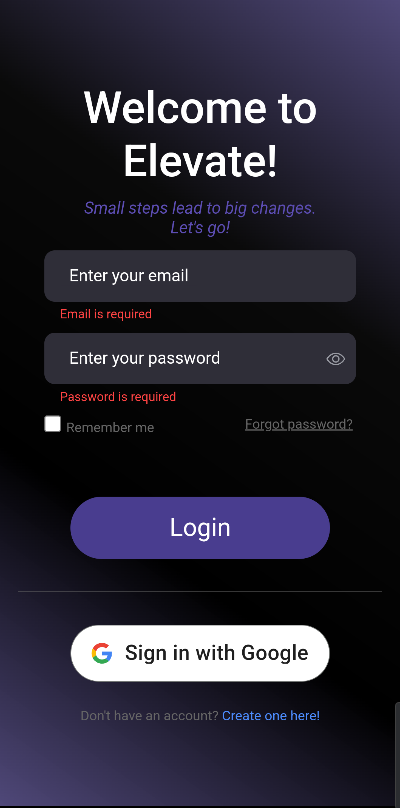
\includegraphics[width=\linewidth]{Képernyőkép 2025-04-15 120810.png}
       1. lépés
    \end{minipage}
    \hfill
    \begin{minipage}[b]{0.23\textwidth}
        \centering
        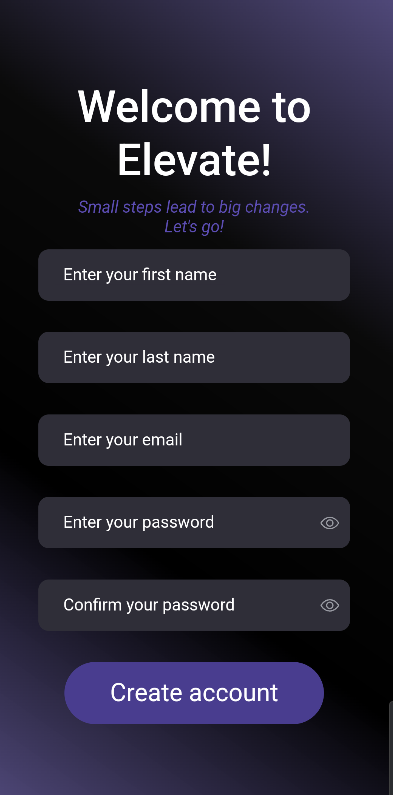
\includegraphics[width=\linewidth]{Képernyőkép 2025-04-15 120821.png}
       2. lépés
    \end{minipage}
    \hfill
    \begin{minipage}[b]{0.23\textwidth}
        \centering
        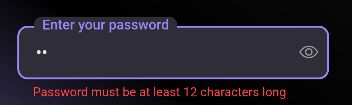
\includegraphics[width=\linewidth]{Képernyőkép 2025-04-15 120848.png}
        3. lépés
    \end{minipage}
    \hfill
    \begin{minipage}[b]{0.23\textwidth}
        \centering
        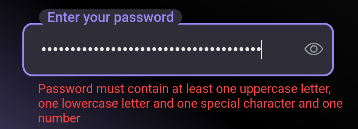
\includegraphics[width=\linewidth]{Képernyőkép 2025-04-15 120855.png}
        4. lépés
    \end{minipage}
   Mobilos bejelentkezés lépései
    \label{fig:login-steps}
\end{figure}

Amennyiben a felhasználó nem rendelkezik fiókkal, meg kell nyomnia a Create one here! gombot.  A sikeres regisztráció után automatikusan átirányítás történik a bejelntkezési oldalra, ahogy be kell jelentkezni a már meglévő fiókkal. Amennyiben a felhasználó rendelkezik fiókkal, nem kell regisztrálnia. Sikeres bejelentkezés után automatikusan átirányítás történik a Szokások (Habits) oldalra
\section{Szokás hozzáadás}
\begin{figure}[H]
    \centering

    % First row - 3 images
    \begin{minipage}[b]{0.25\textwidth}
        \centering
        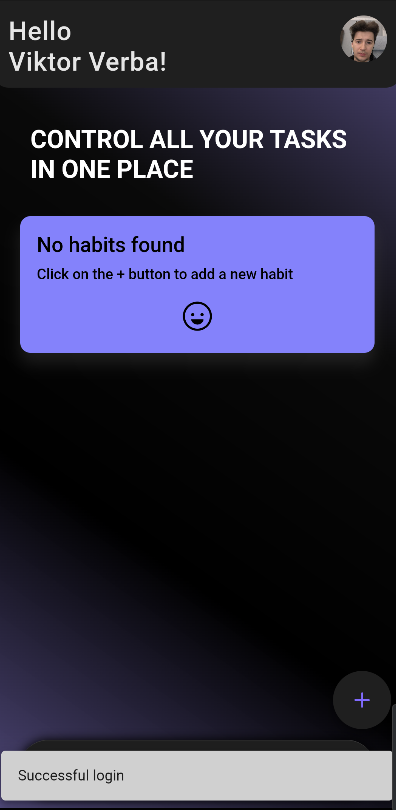
\includegraphics[width=\linewidth]{Képernyőkép 2025-04-15 121001.png}
       Szokás hozzáadása, meg kell nyomni a + gombot
    \end{minipage}
    \hfill
    \begin{minipage}[b]{0.25\textwidth}
        \centering
        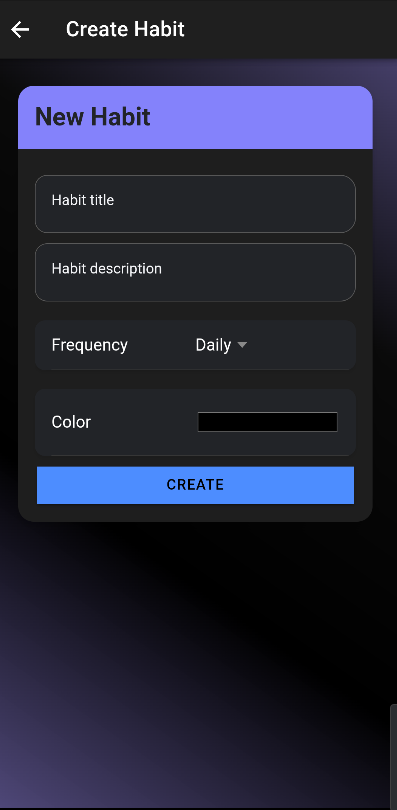
\includegraphics[width=\linewidth]{Képernyőkép 2025-04-15 121459.png}
       Szokás adatainak feltöltése
    \end{minipage}
    \hfill
    \begin{minipage}[b]{0.25\textwidth}
        \centering
        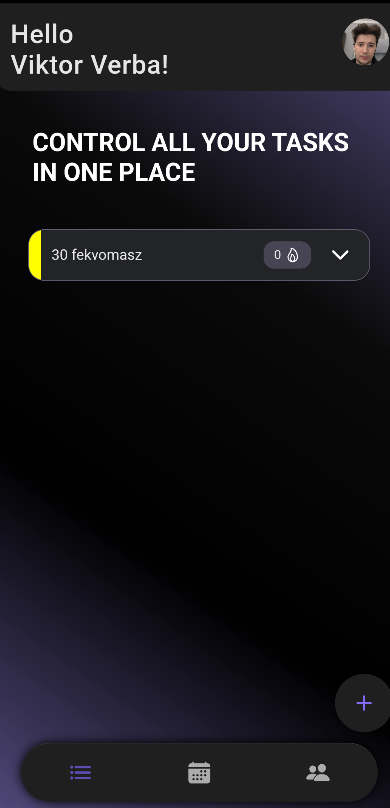
\includegraphics[width=\linewidth]{Képernyőkép 2025-04-15 121610.png}
        Láthatjuk a frissen hozzáadott szokást
    \end{minipage}

    \vspace{0.8em}

    % Second row - 2 images
    \hfill
    \begin{minipage}[b]{0.25\textwidth}
        \centering
        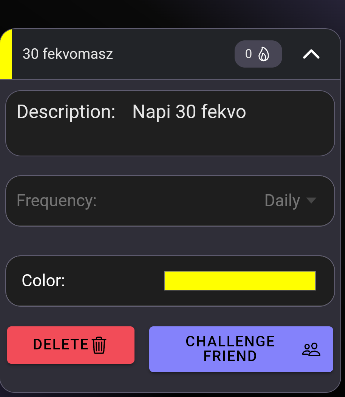
\includegraphics[width=\linewidth]{Képernyőkép 2025-04-15 121618.png}
        Kattintásra kinyílik a szokás
    \end{minipage}

    {Szokás létrehozásának lépései a mobilalkalmazásban}
    \label{fig:habit-creation}
\end{figure}

A fenti képeken látható, hogyan lehet egy új szokást hozzáadni az alkalmazáson belül. A felhasználó kiválasztja a szokás típusát, megadja a nevet, gyakoriságot, majd elmenti azt. Ez segít abban, hogy a napi célkitűzések következetesen teljesüljenek.

\section{Szokás teljesítés}
\begin{figure}[H]
    \centering

    \begin{minipage}[b]{0.3\textwidth}
        \centering
        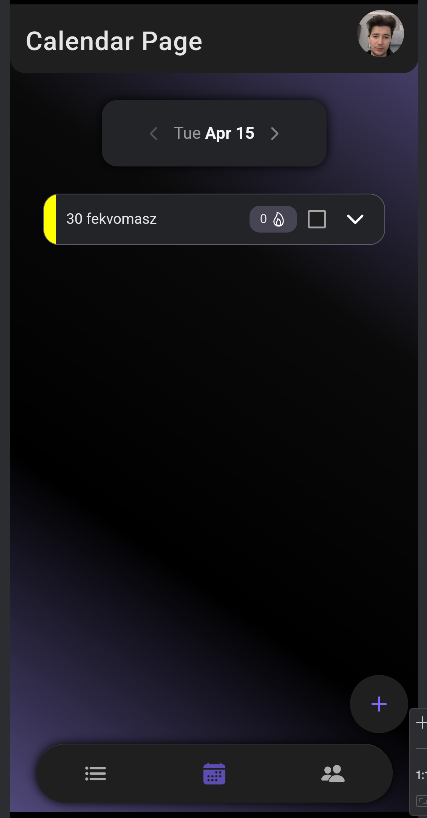
\includegraphics[width=\linewidth]{Képernyőkép 2025-04-15 121644.png}
       Napi nézett, kis kockára kattintva teljesíthető a szokás
    \end{minipage}
    \hfill
    \begin{minipage}[b]{0.3\textwidth}
        \centering
        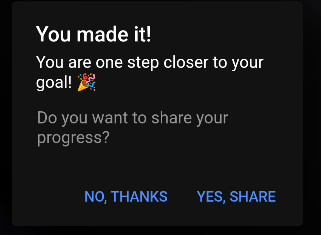
\includegraphics[width=\linewidth]{Képernyőkép 2025-04-15 121704.png}
        Kiválasztás hogy publikus legyen-e a teljesítésünk
    \end{minipage}
    \hfill
    \begin{minipage}[b]{0.3\textwidth}
        \centering
        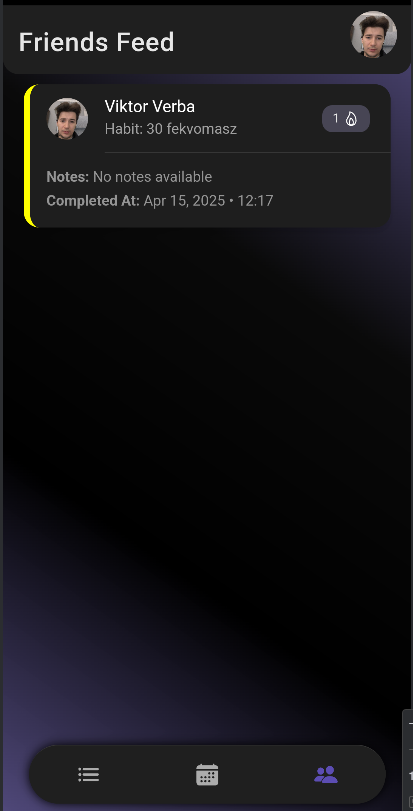
\includegraphics[width=\linewidth]{Képernyőkép 2025-04-15 121715.png}
        Amennyiben publikusat választottunk, a szokás megjelenik a feed oldalon
    \end{minipage}




\end{figure}
  A fenti lépések bemutatják, hogyan lehet egy szokást teljesítettként jelölni a naptár nézetben és megjeleniteni feed-ben. Kalendár nézetben válthatjuk a napokat nyílak segítségével. 

\section{Barátok hozzáadása}
\begin{figure}[H]
    \centering

    % Első sor - 3 kép
    \begin{minipage}[b]{0.25\textwidth}
        \centering
        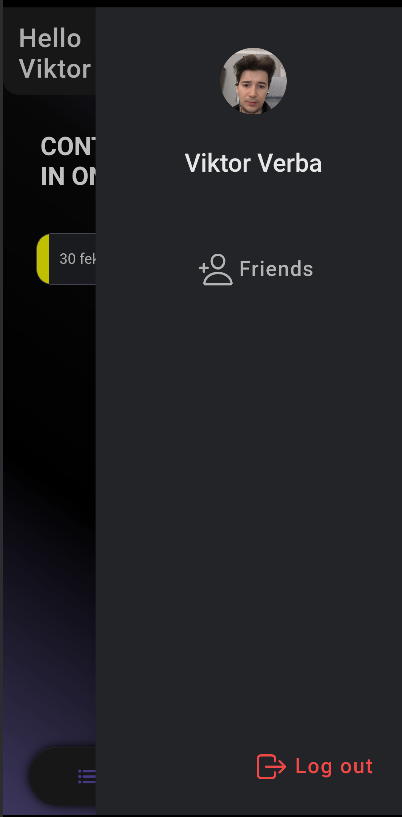
\includegraphics[width=\linewidth]{Képernyőkép 2025-04-15 121728.png}

    \end{minipage}
    \hfill
    \begin{minipage}[b]{0.25\textwidth}
        \centering
        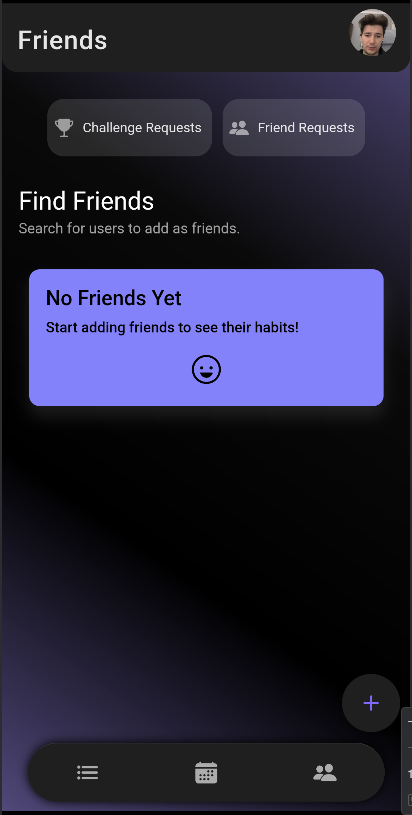
\includegraphics[width=\linewidth]{Képernyőkép 2025-04-15 121737.png}

    \end{minipage}
    \hfill
    \begin{minipage}[b]{0.25\textwidth}
        \centering
        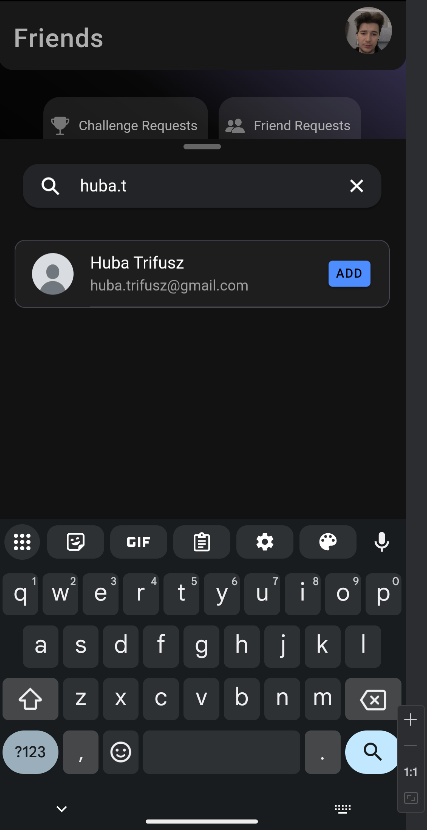
\includegraphics[width=\linewidth]{Képernyőkép 2025-04-15 121807.png}

    \end{minipage}

    \vspace{0.8em} % Kis függőleges térköz a sorok között

    % Második sor - 2 kép
    \begin{minipage}[b]{0.25\textwidth}
        \centering
        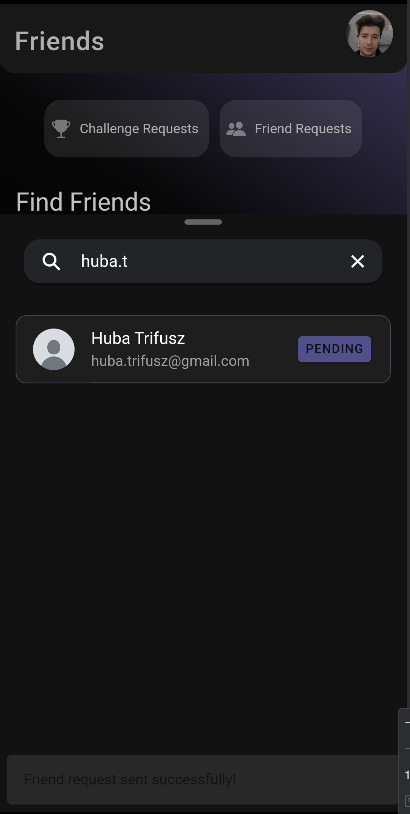
\includegraphics[width=\linewidth]{Képernyőkép 2025-04-15 121821.png}

    \end{minipage} % Üres hely a középső pozícióra
    \begin{minipage}[b]{0.25\textwidth}
        \centering
        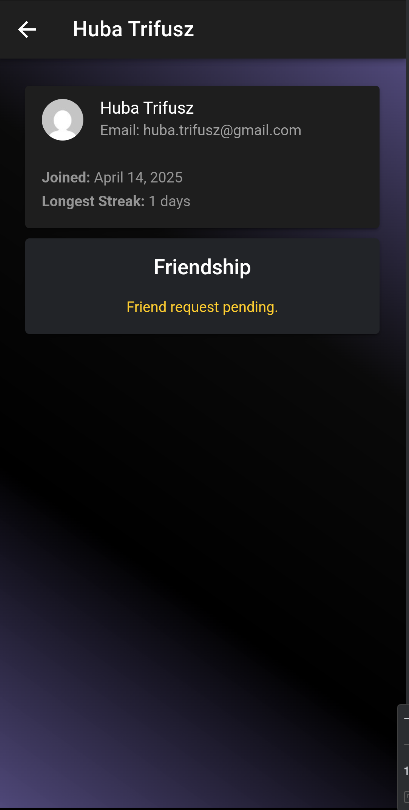
\includegraphics[width=\linewidth]{Képernyőkép 2025-04-15 121842.png}

    \end{minipage}

\end{figure}

    Profileképre kattintva megjelenik a menü, ahogy Friends gombra kattintva átírányit minket a program Barátok oldalra. Itt láthatjuk hogy nincs barátunk, + gombra kattintva kereshetünk a felhasználók között. Miután megtaláltunk a keresett személyt rákattinthatunk az Add gombra.         Miután megnyomtunk a gomb felírata megváltozik. Keresett felhasználó profilképére kattintva megtekinthetjuk a felhasználó összes adatát és azt is hogy a baráti kérelem el lett küldve.

\section{Baráti kérelem fogadás}
\begin{figure}[H]
    \centering

    % Felső sor - 3 kép
    \begin{minipage}[t]{0.25\textwidth}
        \centering
        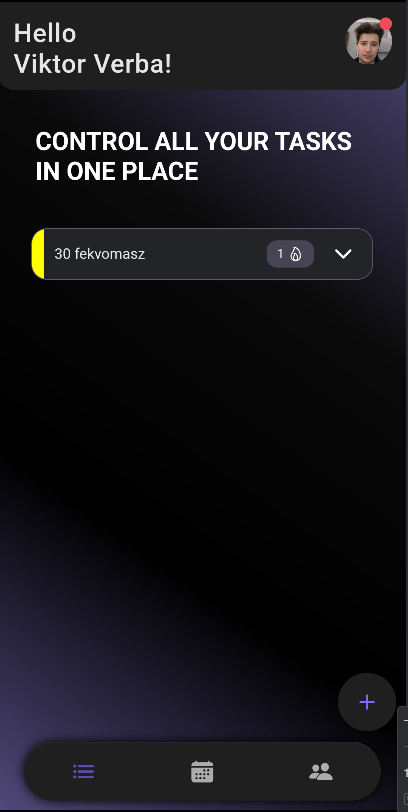
\includegraphics[width=\linewidth]{Képernyőkép 2025-04-15 122022.png}
    \end{minipage}
    \hfill
    \begin{minipage}[t]{0.25\textwidth}
        \centering
        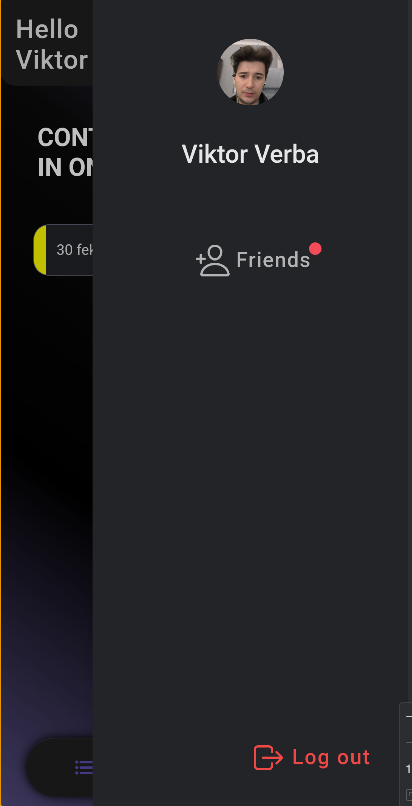
\includegraphics[width=\linewidth]{Képernyőkép 2025-04-15 122051.png}
    \end{minipage}
    \hfill
    \begin{minipage}[t]{0.25\textwidth}
        \centering
        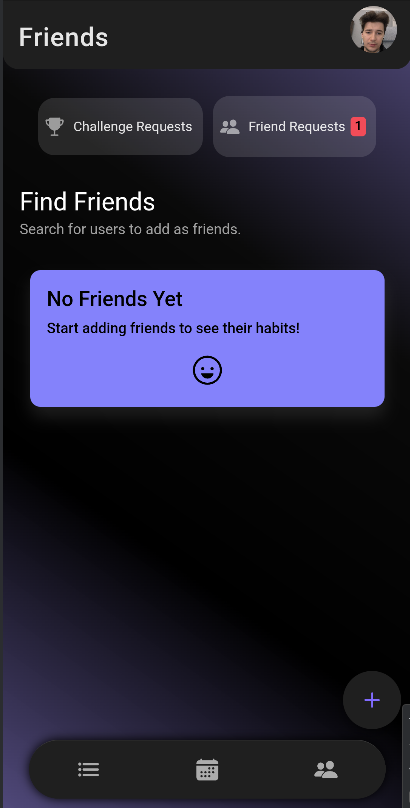
\includegraphics[width=\linewidth]{Képernyőkép 2025-04-15 122102.png}
    \end{minipage}

    \vspace{0.8em}

    % Alsó sor - 2 kép
    \begin{minipage}[t]{0.25\textwidth}
        \centering
        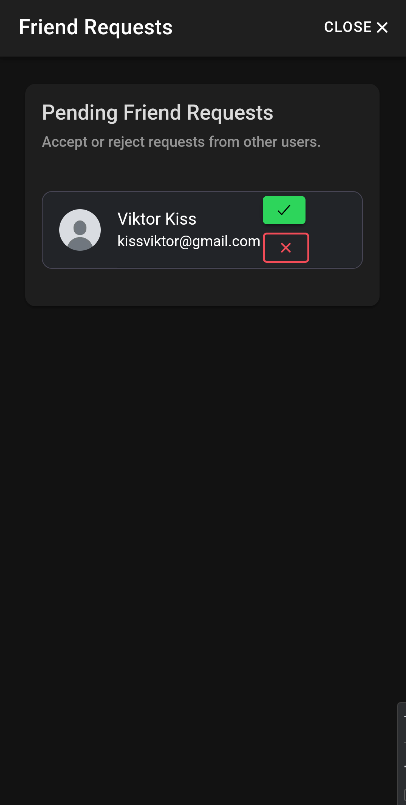
\includegraphics[width=\linewidth]{Képernyőkép 2025-04-15 122115.png}
    \end{minipage}
    \hfill
    \begin{minipage}[t]{0.25\textwidth}
        \centering
        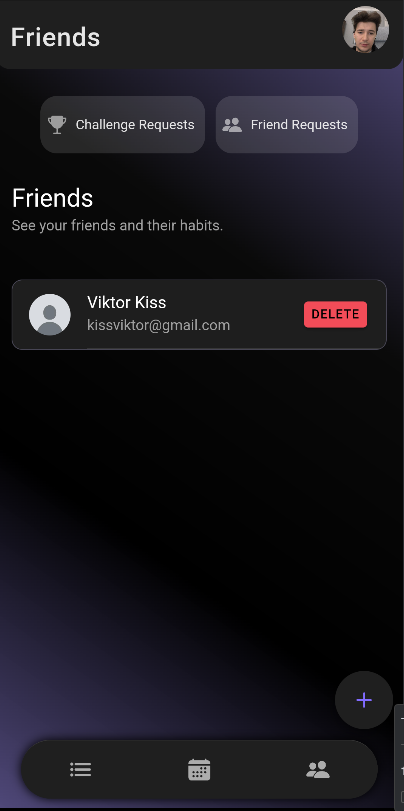
\includegraphics[width=\linewidth]{Képernyőkép 2025-04-15 122133.png}
    \end{minipage}


\end{figure}
  Amennyiben a program észlel, hogy valaki küldött nekünk baráti kérelmet vagy challenge kérelmet a profilképnél megjeleník egy kis piros pötty. Miután rákattintunk a profilképünkre a Friends gombon is látni fogjuk a pöttyöt, ami azt jelzi, hogy ezen az oldalon érkezett kérelem. Miután barátok oldalra lépünk láthatjuk a baráti kérelem és challenge gombokat. Piros szám azt jelzi hogy hány kérelem érkezett hozzánk. Friend Requests gombra kattintva megjelennek a beérkezett baráti kérelmek. Elfogadás után a barátunk megjelenik a listában.
\section{Kihívás}
% Első oldal - 6 kép
\begin{figure}[H]
    \centering

    % 1. sor
    \begin{minipage}[b]{0.25\textwidth}
        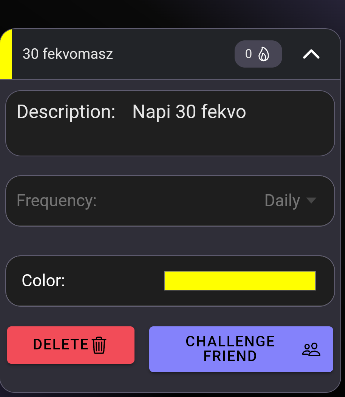
\includegraphics[width=\linewidth]{Képernyőkép 2025-04-15 121618.png}
    \end{minipage}
    \hfill
    \begin{minipage}[b]{0.25\textwidth}
        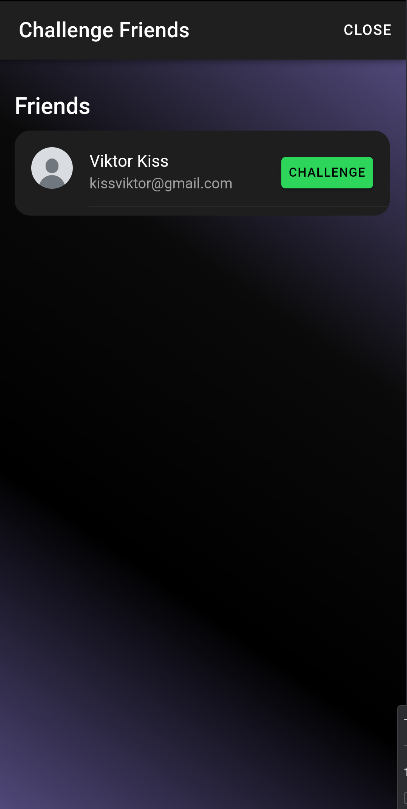
\includegraphics[width=\linewidth]{Képernyőkép 2025-04-15 122147.png}
    \end{minipage}
    \hfill
    \begin{minipage}[b]{0.25\textwidth}
        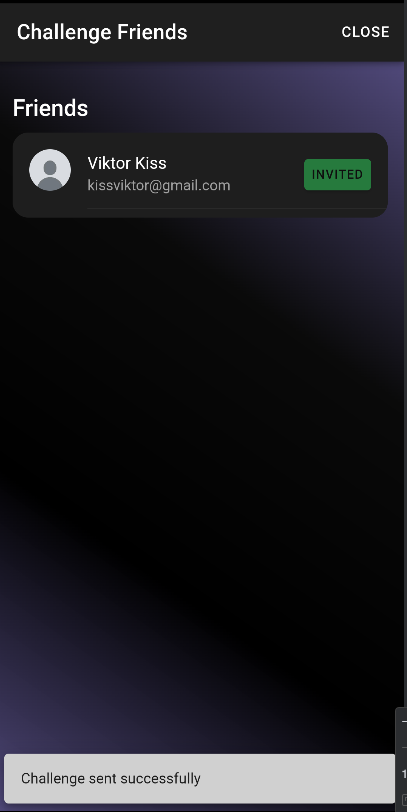
\includegraphics[width=\linewidth]{Képernyőkép 2025-04-15 122156.png}
    \end{minipage}

    \vspace{0.8em}

    % 2. sor
    \begin{minipage}[b]{0.25\textwidth}
        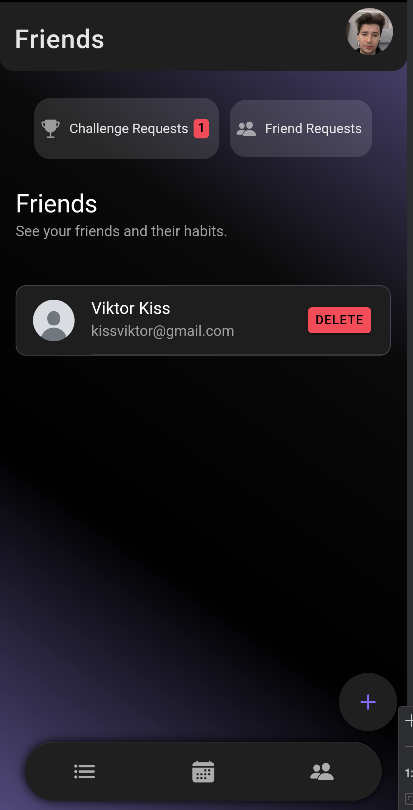
\includegraphics[width=\linewidth]{Képernyőkép 2025-04-15 122257.png}
    \end{minipage}
    \hfill
    \begin{minipage}[b]{0.25\textwidth}
        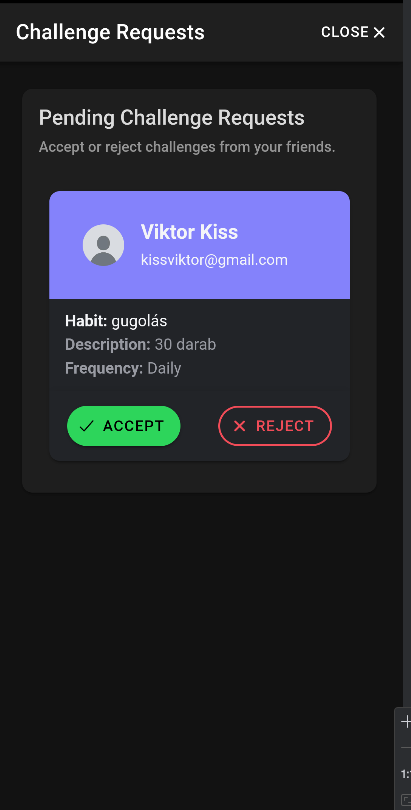
\includegraphics[width=\linewidth]{Képernyőkép 2025-04-15 122306.png}
    \end{minipage}
    \hfill
    \begin{minipage}[b]{0.25\textwidth}
        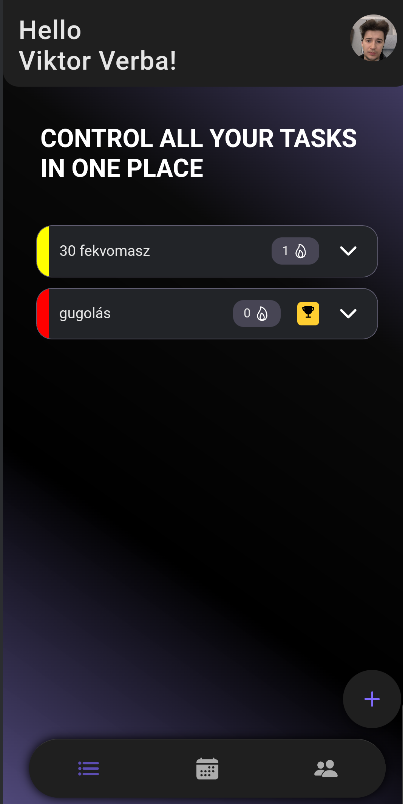
\includegraphics[width=\linewidth]{Képernyőkép 2025-04-15 122327.png}
    \end{minipage}
\end{figure}

\newpage

% Második oldal - 3 kép
\begin{figure}[H]
    \centering

    % 3. sor
    \begin{minipage}[b]{0.3\textwidth}
        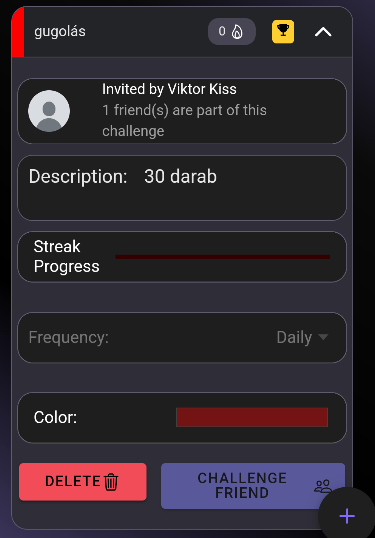
\includegraphics[width=\linewidth]{Képernyőkép 2025-04-15 122343.png}
    \end{minipage}
    \hfill
    \begin{minipage}[b]{0.3\textwidth}
        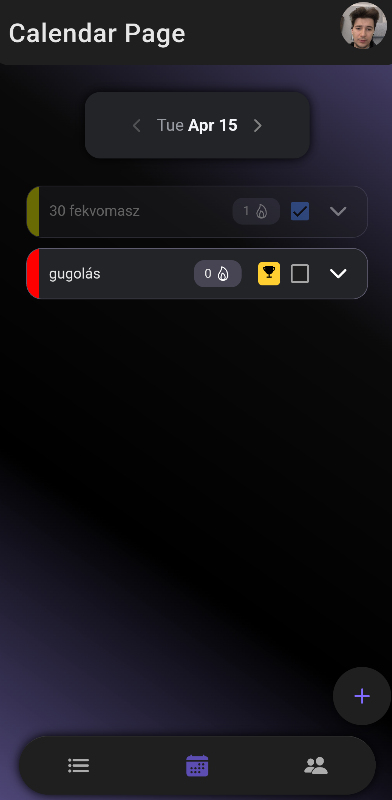
\includegraphics[width=\linewidth]{Képernyőkép 2025-04-15 122358.png}
    \end{minipage}
    \hfill
    \begin{minipage}[b]{0.3\textwidth}
        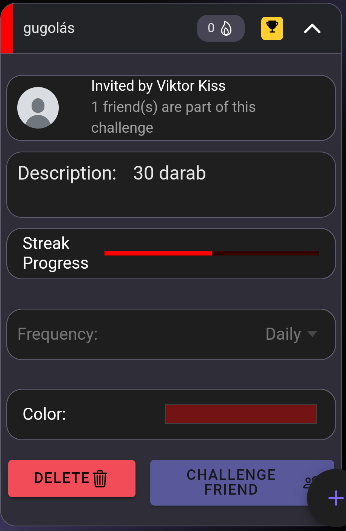
\includegraphics[width=\linewidth]{Képernyőkép 2025-04-15 122424.png}

    \end{minipage}
\end{figure}
    \footnotesize Amennyiben a felhasználó rendelkezik barátokkal, akkor tud küldeni a barátainak kihívást (challenget) amit onnantól közösen kell elvégezniuk ahhoz, hogy a streak nőjőn. Szokásra kattintva rá kell kattintani a Challenge friend gombra, amely átvisz egy oldalra, ahol kiválaszthatjuk a barátot, akit meg akarjuk hívni. Miután rákattintottunk a challenge gombra, kapunk visszajelzést és a gomb átváltozik Invited-re. További képeken látható, hogy kell elfogadni vagy elutasítani a kihívásokat. Amennyiben elfogadjuk a kihívást az meg fog jelenni a szokásaink közül. Kihívást egy kis ikonnal tudunk megkülönböztetni. Ha valaki meghívott minket, akkor láthatjuk ki volt az és hányan vesznek részt benne. Streak Progress mutatja, hogy eddig hányan teljesítették a resztvevők közül a kihívást.



\section{Profilkép}
\begin{figure}[H]
    \centering

    \begin{minipage}[b]{0.3\textwidth}
        \centering
        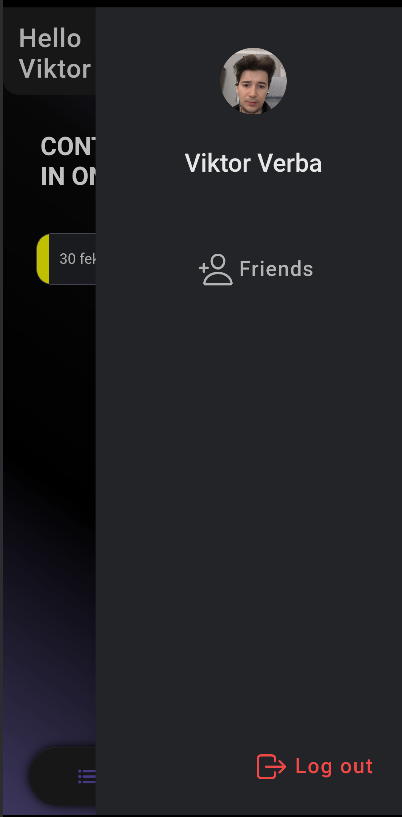
\includegraphics[width=\linewidth]{Képernyőkép 2025-04-15 121728.png}
        \par
        \footnotesize Profileképre kattintva átvisz minket a profil oldalra. 
    \end{minipage}
    \hfill
    \begin{minipage}[b]{0.3\textwidth}
        \centering
        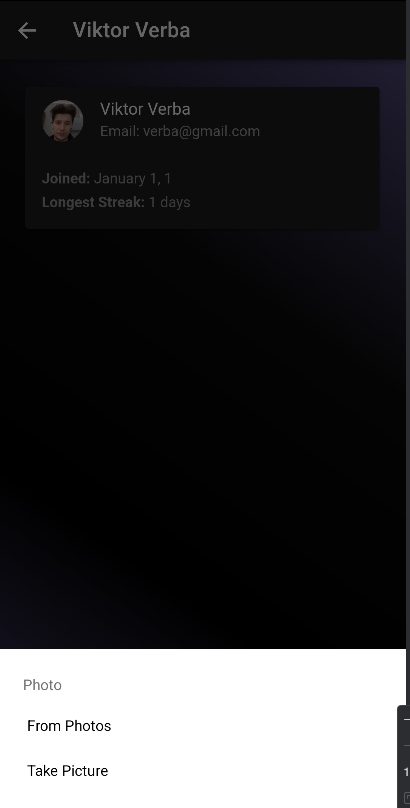
\includegraphics[width=\linewidth]{Képernyőkép 2025-04-15 145953.png}
        \par
        \footnotesize Profilképre kattintva kiválaszthatjuk, hogy képek közül akarunk választani vagy csinálni akarunk egy képet.
    \end{minipage}
    \hfill
    \begin{minipage}[b]{0.3\textwidth}
        \centering
        \includegraphics[width=\linewidth]{Képernyőkép 2025-04-15 150008.png}
        \par
        \footnotesize Képcsinálásra megnyílik a kamera
    \end{minipage}


\end{figure}
\end{document}